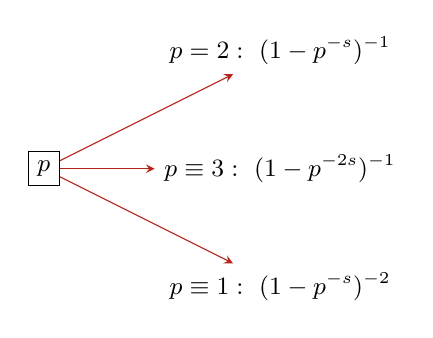
\begin{tikzpicture}[>=stealth,font=\small]
\node[draw] (a) at (0,0) {$p$};
\node (b) at (3,1.5) {$p=2:\ (1-p^{-s})^{-1}$};
\node (c) at (3,0) {$p\equiv3:\ (1-p^{-2s})^{-1}$};
\node (d) at (3,-1.5) {$p\equiv1:\ (1-p^{-s})^{-2}$};
\draw[->,BrickRed] (a)--(b);\draw[->,BrickRed] (a)--(c);\draw[->,BrickRed] (a)--(d);
\end{tikzpicture}
